\documentclass[12pt]{article}

\usepackage[utf8x]{inputenc}
\usepackage[L7x, T2A]{fontenc}
\usepackage[lithuanian]{babel}
\usepackage{vwcol}  
\usepackage{sectsty}
\usepackage{setspace}
\usepackage{fancyhdr}
\usepackage{graphicx}
\usepackage{ragged2e}
\usepackage{titlesec}
\usepackage{epsfig}
\usepackage{indentfirst}
\usepackage[top=2cm, bottom=2cm, left=3cm, right=1.5cm]{geometry}
\usepackage{makecell}
\usepackage[justification=centering]{caption}
\usepackage{titlesec}
\usepackage{fullpage}
\usepackage{amsmath,amssymb,amsthm,enumitem}
\usepackage{enumitem}
\usepackage{color}  
\usepackage{hyperref}
\hypersetup{
    colorlinks=true,
    linktoc=all,
    linkcolor=black,
}
\usepackage[tocindentauto]{tocstyle}
\usetocstyle{standard}

\usepackage{svg}

\makeatletter
\expandafter\let\csname L7x-cmd\endcsname\@changed@cmd
\makeatother

\addto\extraspolish{\fontencoding{L7x}\selectfont}
\addto\noextraspolish{\fontencoding{\encodingdefault}\selectfont}

\setlength\parindent{1cm}

\title{VILNIAUS UNIVERSITETAS \\
MATEMATIKOS IR INFORMATIKOS FAKULTETAS \\
PROGRAMŲ SISTEMŲ KATEDRA}
\author{}
\date{}

\pagestyle{fancy}
\fancyhead{}
\fancyfoot{}
\fancyfoot[R]{\thepage}
\renewcommand{\headrulewidth}{0pt}
\renewcommand{\baselinestretch}{1.5}


\renewcommand{\thesubsection}{FR\arabic{subsection}}
\renewcommand*{\theenumi}{\thesubsection.\arabic{enumi}}
\renewcommand*{\theenumii}{\thesubsubsection.\theenumi.\arabic{enumii}}

%\titleformat{\subsection}{\Large\bfseries}{\arabic{subsection}}{1em}{}
\titleformat{\subsubsection}{\bfseries}{\thesubsection.\arabic{subsubsection}}{1em}{}

\begin{document}
	\clearpage
	\maketitle
	\thispagestyle{empty}

	\bigbreak
	\bigbreak
	\bigbreak
	\bigbreak

	\begin{center}
		\begin{Large}
			\textbf{Transporto priemonių skelbimų aplikacija} \\
		\end{Large}
		\begin{large}
			\textbf{Application for Vehicle Advertisement} \\
		\end{large}
		Programų sistemų inžinerijos I laboratorinis darbas Nr. 2 \\

		\bigbreak
		\bigbreak
		\bigbreak
		\bigbreak
		\bigbreak
		\bigbreak
		\bigbreak
		\bigbreak
		\bigbreak

		\begin{tabular}{ll}
			Atliko:        & 2 kurso 5 grupės studentai \\
		               	   & Toma Burneikaitė \\
		               	   & Žygimantas Stongvilas \\
		                   & Mantas Jurčius \\
		                   & Rimvydas Meškauskas \\
			Darbo vadovas: & asist., dr., Vytautas Valaitis
		\end{tabular}

		\bigbreak
		\bigbreak
		\bigbreak
		\bigbreak
		\bigbreak
		\bigbreak
		\bigbreak
		\bigbreak
		\bigbreak

		Vilnius - 2018
	\end{center}
	\pagebreak
	
	\tableofcontents
	\pagebreak	
	
	\section*{Funkciniai reikalavimai}
	\addcontentsline{toc}{section}{Funkciniai reikalavimai}
	
	\subsection{Bendri reikalavimai}
	\begin{enumerate}[labelindent=10pt,leftmargin=2.2cm]
		\item Įrenginys, kuriame naudojama programinė sistema, turi turėti prieigą prie interneto.
		\item Programinės įrangos įdiegimas turi būti laisvai prieinamas visiems norintiems ja naudotis.
		\item Vartotojas turės galimybę keisti savo asmeninius duomenis (vartotojo vardą ir slaptažodį).
		\item Skelbimai, pridėti prie mėgstamiausių sąrašo, bus saugomi vartotojo įrenginyje.
		\item Valiutų kursai nustatomi remiantis Lietuvos Banko duomenimis.
		\item Sistema vartotojui neprisijungus leis atlikti jos pagrindines funkcijas (skelbimų paieška).
		\item Sistema vartotojui prisijungus leis atlikti pagrindines (skelbimų paieška) ir papildomas funkcijas (mėgstamiausių sąrašas).
		\item Mėgstamiausių sąrašas atitinkamam vartotojui bus prieinamas tik jam ir niekam kitam.
		\item Sistema vartotojui leis iš bet kurio jos lango grįžti į pagrindinį langą.
	\end{enumerate}
	
	\subsection{Užsakovo reikalavimai}
	\begin{enumerate}[labelindent=10pt,leftmargin=2.2cm]
		\item Sistemos savininkas turi visas įmanomas sistemos teises (savas bei administratoriaus ir kliento).
		\item Sistemos savininkas gali paskirti naujus administratorius bei pašalinti esamus (suteikti arba atimti administratoriaus teises).
	\end{enumerate}	
	\pagebreak
	
	\renewcommand*{\theenumi}{\thesubsubsection.\arabic{enumi}}
	\renewcommand*{\theenumii}{\thesubsubsection.\theenumi.\arabic{enumii}}
	\renewcommand*{\theenumiii}{\thesubsubsection.\theenumi.\theenumii.\arabic{enumiii}}
	\subsection{Vartotojo reikalavimai}\label{Vartotojo_reikalavimai}
	Šiame skyriuje nagrinėjami vartotojui aktualūs reikalavimai sistemai „AutoINF“. Pateikiami vartotojo funkciniai reikalavimai, užduočių scenarijai bei jų plėtiniai.
	
	\begin{figure}[h]
		\begin{center}
			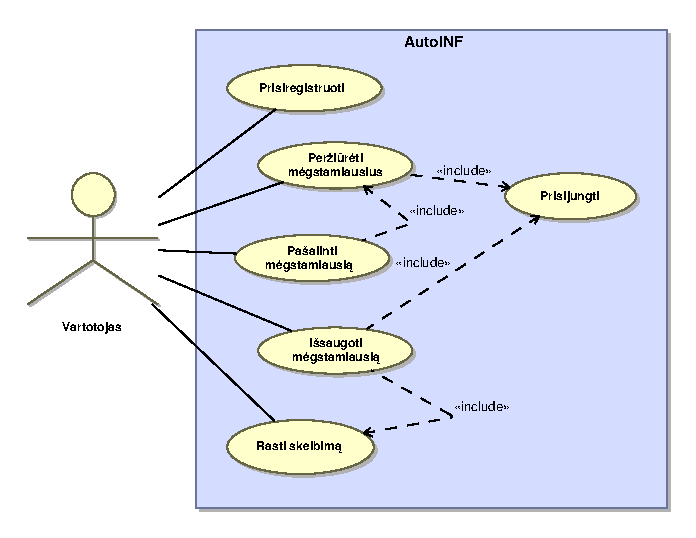
\includegraphics[width=0.7\textwidth]{TikslaiVartotojas.eps}
			\caption{Sistemos užduočių diagrama iš vartotojo perspektyvos\label{UseCaseUser}}
		\end{center}
	\end{figure}
	\pagebreak
	
	\subsubsection{Pagrindinio meniu reikalavimai}
	\begin{enumerate}[labelindent=10pt,leftmargin=2.2cm]
		\item Pagrindiniame lange vartotojas, jei jis neprisijungęs, turi galimybę pasinaudoti sistemos funkcijomis: prisiregistruoti, prisijungti bei ieškoti skelbimų.
	\end{enumerate}
		
		\begin{center}
		\captionof{table}{Pagrindinio lango scenarijus, kai vartotojas nėra prisijungęs\label{UserNotLoggedIn}}
		\begin{tabular}{ | c | c | c | }
			\hline
			Žingsnis & Aktorius   & Veiklos apibūdinimas \\ \hline
			1        & Aplikacija & \makecell{Paprašo pasirinkti norimą veiksmą: \\ Prisiregistruoti \\ Prisijungti \\ Rasti skelbimą} \\ \hline
			2        & Vartotojas & Pasirenka veiksmą \\ \hline
			3        & Aplikacija & Įvykdo pasirinktą veiksmą \\ \hline
		\end{tabular}
		\bigskip
		\end{center}
		
	\begin{enumerate}[resume, labelindent=10pt,leftmargin=2.2cm]
		\item Pagrindiniame lange vartotojas, jei jis prisijungęs, turi galimybę pasinaudoti šiomis sistemos funkcijomis: ieškoti skelbimų, peržiūrėti mėgstamiausius (registracijos mygtuko nebelieka).
	\end{enumerate}
		
		\begin{center}
		\captionof{table}{Pagrindinio lango scenarijus, kai vartotojas yra prisijungęs\label{UserLoggedIn}}		
		\begin{tabular}{ | c | c | c | }
			\hline
			Žingsnis & Aktorius   & Veiklos apibūdinimas \\ \hline
			1        & Aplikacija & \makecell{Paprašo pasirinkti norimą veiksmą: \\ Peržiūrėti mėgstamiausius \\ Pašalinti mėgstamiausią \\ Išsaugoti mėgstamiausią \\ Rasti skelbimą} \\ \hline
			2        & Vartotojas & Pasirenka veiksmą \\ \hline
			3        & Aplikacija & Įvykdo pasirinktą veiksmą \\ \hline
		\end{tabular}
		\bigskip
		\end{center}		
		
	\begin{enumerate}[resume, labelindent=10pt,leftmargin=2.2cm]
		\item Pagrindiniame lange turi būti pavaizduotas filtras, pagal kurį vartotojas gali ieškoti skelbimų.
	\end{enumerate}	
	\pagebreak
	
	\subsubsection{Vartotojo prisiregistravimo reikalavimai}
	\begin{enumerate}[labelindent=10pt,leftmargin=2.2cm]
		\item Vartotojas, norintis prisiregistruoti, turi būtinai būti užpildęs registracijai reikiamus laukus. Jei paspaudus registracijos mygtuką kurie nors privalomi laukai yra palikti neužpildyti, tie laukai yra paryškinami raudonai ir šalia parodomas pranešimas, kad kai kurie registracijos laukai yra neužpildyti.
	\end{enumerate}
		
		\begin{center}
		\captionof{table}{Vartotojo registracijos scenarijus\label{UserRegScen}}		
		\begin{tabular}{ | c | c | c | }
			\hline
			Žingsnis & Aktorius     & Veiklos apibūdinimas \\ \hline
			1        & Aplikacija   & Paprašo pasirinkti norimą veiksmą \\ \hline
			2        & Vartotojas   & Pasirenka registraciją \\ \hline
			3        & Aplikacija   & Atidaro registracijos langą \\ \hline
			4        & Vartotojas   & \makecell{Suveda prisiregistravimo duomenis ir \\ spaudžia mygtuką „Prisiregistruoti“} \\ \hline
			5        & Aplikacija   & \makecell{Patikrina duomenų formato teisingumą ir \\ siunčia duomenis į serverį} \\ \hline
			6        & Serveris     & Siunčia užklausą į duomenų bazę \\ \hline
			7        & Duomenų bazė & Perspėja serverį apie (ne)sėkmingą registraciją \\ \hline
			8        & Serveris     & Perspėja aplikaciją apie (ne)sėkmingą registraciją \\ \hline
			9        & Aplikacija   & \makecell{Parodo pranešimą apie registracijos (ne)sėkmingumą ir \\ perkrauna pagrindinį langą su prisijungusio vartotojo \\ interfeisu bei laukia, kol vartotojas atliks kitą veiksmą} \\ \hline
		\end{tabular}
		\bigskip
		\end{center}	
		
	\begin{enumerate}[resume, labelindent=10pt,leftmargin=2.2cm]
		\item Registracijos laukai turi būti užpildyti reikiamu formatu (pvz., el. paštas -> test@mail.lt). Jei kurie nors laukai yra užpildyti neteisingu formatu, tai paspaudus registracijos mygtuką šitie laukai yra paryškinami raudonai ir šalia parodomas pranešimas, kad kai kurie laukai užpildyti neteisingai.
		\pagebreak
		\item Teisingai suvedus duomenis ir vartotojui paspaudus registracijos mygtuką sistema turi patikrinti, ar paskyra su tokiais duomenimis neegzistuoja, siekiant užtikrinti, kad nebūtų kelių paskyrų su tokiais pačiais el. paštais ar vartotojų vardais. Patikrinimui pasibaigus parodomas pranešimas apie registracijos (ne)sėkmingumą.	
	\end{enumerate}
		
		\begin{center}
		\captionof{table}{Vartotojo registracijos scenarijaus plėtiniai\label{UserRegScenExtra}}		
		\begin{tabular}{ | c | c | c | }
			\hline
			Žingsnis & Sąlyga                                     & Veiklos apibūdinimas \\ \hline
			5a       & \makecell{Neteisingas \\ duomenų formatas} & \makecell{Klaidingai užpildyti laukai yra paryškinami raudonai \\ ir parodomas pranešimas, kad kai kurie \\ registracijos laukai yra užpildyti klaidingai} \\ \hline
			5b       & \makecell{Palikti \\ neužpildyti laukai}   & Neužpildyti laukai yra paryškinami raudonai \\ \hline
			7a       & \makecell{Duomenų bazėje \\ nepavyko išsaugoti \\ duomenų} & Parodomas pranešimas apie nesėkmingą registraciją \\ \hline
		\end{tabular}
		\end{center}
	\pagebreak
	
	\subsubsection{Vartotojo prisijungimo reikalavimai}
	\begin{enumerate}[labelindent=10pt,leftmargin=2.2cm]
		\item Vartotojui paspaudus prisijungimo mygtuką, sistema turi patikrinti, ar prisijungimo laukai užpildyti. Jei ne, vartotojui parodomas pranešimas, kad prisijungimo laukai palikti tušti.
	\end{enumerate}
		
		\begin{center}
		\captionof{table}{Vartotojo prisijungimo scenarijus\label{UserLogInScen}}		
		\begin{tabular}{ | c | c | c | }
			\hline
			Žingsnis & Aktorius     & Veiklos apibūdinimas \\ \hline
			1        & Vartotojas   & Pasirenka prisijungimo funkciją \\ \hline
			2        & Aplikacija   & Parodo prisijungimo langą \\ \hline
			3        & Vartotojas   & Suveda prisijungimo duomenis \\ \hline
			4        & Vartotojas   & Jungiasi su įvestais duomenimis \\ \hline
			5        & Aplikacija   & Siunčia užklausą į serverį \\ \hline
			6        & Serveris     & Siunčia užklausą į duomenų bazę \\ \hline
			7        & Duomenų bazė & Praneša serveriui apie sėkmingą prisijungimą \\ \hline
			8        & Serveris     & Praneša aplikacijai apie sėkmingą prisijungimą \\ \hline
			9        & Aplikacija   & \makecell{Parodo pagrindinį langą su papildomomis \\ prisijungusio vartotojo funkcijomis} \\ \hline
		\end{tabular}
		\bigskip
		\end{center}
		
	\begin{enumerate}[resume, labelindent=10pt,leftmargin=2.2cm]
		\item Jei prisijungimo laukai užpildyti, tai sistema patikrina, ar toks vartotojas egzistuoja. Jei vartotojo vardas ir slaptažodis įvesti teisingai, tai sistema perkrauną pagrindinį langą su prisijungusio vartotojo interfeisu. Jei vartotojo vardas ir slaptažodis įvesti neteisingai, tai vartotojui yra pranešama apie neteisingai suvestus duomenis.
	\end{enumerate}		
		
		\begin{center}
		\captionof{table}{Vartotojo prisijungimo scenarijaus plėtiniai\label{UserLogInScenExtra}}		
		\begin{tabular}{ | c | c | c | }
			\hline
			Žingsnis & Sąlyga                                     & Veiklos apibūdinimas \\ \hline
			4a       & \makecell{Vartotojas neužpildė \\ visų prisijungimo laukų} & Neužpildyti laukai yra paryškinami raudonai \\ \hline
			7a       & \makecell{Suvesti klaidingi \\ prisijungimo duomenys} & Parodomas pranešimas apie nesėkmingą prisijungimą \\ \hline
		\end{tabular}
		\end{center}
	\pagebreak
	
	\subsubsection{Vartotojo skelbimų ieškojimo reikalavimai}
	\begin{enumerate}[labelindent=10pt,leftmargin=2.2cm]
		\item Vartotojui teisingai suvedus paieškos kriterijus ir paspaudus paieškos mygtuką, aplikacija turi ekrane parodyti visus rastus skelbimus, atitinkančius filtrą. Sistemai nesugebėjus rasti filtrą atitinkančių skelbimų, ekrane parodomas pranešimas, kad nepavyko rasti užklausą atitinkančių rezultatų.
	\end{enumerate}
		
		\begin{center}
		\captionof{table}{Vartotojo skelbimų ieškojimo scenarijus\label{UserSearchScen}}		
		\begin{tabular}{ | c | c | c | }
			\hline
			Žingsnis & Aktorius     & Veiklos apibūdinimas \\ \hline
			1        & Vartotojas   & \makecell{Vartotojas įveda paieškos kriterijus ir \\ paspaudžia mygtuką „Ieškoti“} \\ \hline
			2        & Aplikacija   & Siunčia užklausą į serverį \\ \hline
			3        & Serveris     & Siunčia užklausą į paieškos modulį \\ \hline
			4        & Paieškos modulis & Grąžina serveriui rastus skelbimus \\ \hline
			5        & Serveris     & Grąžina aplikacijai rastus skelbimus  \\ \hline
			6        & Aplikacija   & Parodo rastų skelbimų sąrašą \\ \hline
			7        & Vartotojas   & Paspausžia ant skelbimo \\ \hline
			8        & Aplikacija   & Atidaro skelbimo langą \\ \hline
		\end{tabular}
		\bigskip

		\captionof{table}{Vartotojo skelbimų ieškojimo scenarijaus plėtiniai\label{UserSearchScenExtra}}		
		\begin{tabular}{ | c | c | c | }
			\hline
			Žingsnis & Sąlyga                                     & Veiklos apibūdinimas \\ \hline
			1a       & \makecell{Vartotojas nesuveda \\ paieškos kriterijų} & \makecell{Vartotojas įspėjamas, kad negalima \\ palikti neužpildytų privalomų laukų} \\ \hline
			5b       & Nerasta skelbimų                           & \makecell{Parodomas pranešimas, kad nėra skelbimų, \\ atitinkančių nurodytą filtrą, ir vartotojas yra \\ grąžinamas į pagrindinį langą } \\ \hline
			7a       & \makecell{Vartotojas nepaspaudžia \\ ant skelbimo} & \makecell{Aplikacija laukia, kol bus paspausta ant \\ skelbimo arba kol vartotojas ieškos naujų \\  skelbimų pagal kitą filtrą} \\ \hline
		\end{tabular}
		\end{center}
	
	\subsubsection{Vartotojo mėgstamiausių skelbimų peržiūrėjimo reikalavimai}
	\begin{enumerate}[labelindent=10pt,leftmargin=2.2cm]
		\item Vartotojui paspaudus „Peržiūrėti mėgstamiausius“ mygtuką parodomas mėgstamiausių skelbimų sąrašas.
	\end{enumerate}
		
		\begin{center}
		\captionof{table}{Vartotojo mėgstamiausių skelbimų peržiūrėjimo scenarijus\label{UserViewFavScen}}		
		\begin{tabular}{ | c | c | c | }
			\hline
			Žingsnis & Aktorius     & Veiklos apibūdinimas \\ \hline
			1        & Vartotojas   & Prisijungia prie sistemos \\ \hline
			2        & Aplikacija   & \makecell{Atidaro pagrindinį langą su papildomomis, \\ registruoto vartotojo, funkcijomis} \\ \hline
			3        & Vartotojas   & Pasirenka „Peržiūrėti mėgstamiausius“ funkciją \\ \hline
			4        & Aplikacija   & Siunčia užklausą į serverį \\ \hline
			5        & Serveris     & Siunčia užklausą į duomenų bazę \\ \hline
			6        & Duomenų bazė & Siunčia serveriui vartotojo mėgstamiausių skelbimų sąrašą \\ \hline
			7        & Serveris     & Siunčia aplikacijai vartotojo mėgstamiausių skelbimų sąrašą \\ \hline
			8        & Aplikacija   & \makecell{Atidaro naują langą su vartotojo išsaugotais \\ jo mėgstamiausiais skelbimais } \\ \hline
		\end{tabular}
		\end{center}
	\pagebreak
	
	\subsubsection{Vartotojo mėgstamiausio skelbimo pašalinimo reikalavimai}
	\begin{enumerate}[labelindent=10pt,leftmargin=2.2cm]
		\item Vartotojui paspaudus mygtuką „Trinti“ aplikacija išmeta papildomą sisteminį langą, kuriame klausiama vartotojo, ar jis tikrai nori panaikinti šį skelbimą iš savo mėgstamiausių sąrašo. Paspaudus „Taip“ skelbimas sėkmingai panaikinamas iš mėgstamiausių sąrašo. 
	\end{enumerate}
		
		\begin{center}
		\captionof{table}{Vartotojo mėgstamiausio skelbimo pašalinimo scenarijus\label{UserRemoveAdScen}}
		\begin{tabular}{ | c | c | c | }
			\hline
			Žingsnis & Aktorius       & Veiklos apibūdinimas \\ \hline
			1        & Vartotojas     & Pasirenka mėgstamiausių skelbimų langą \\ \hline
			2        & Aplikacija     & \makecell{Atidaro mėgstamiausių skelbimų langą ir \\ laukia tolesnių vartotojo veiksmų} \\ \hline
			3        & Vartotojas     & Pasirenka skelbimo šalinimą \\ \hline
			4        & Aplikacija     & Siunčia užklausą į serverį \\ \hline
			5        & Serveris       & Siunčia užklausą į duomenų bazę  \\ \hline
			6        & Duomenų bazė   & \makecell{Pašalina mėgstamiausią skelbimą iš duomenų bazės \\ ir grąžina pranešimą apie sėkmingai pašalintą skelbimą} \\ \hline
			7        & Serveris       & \makecell{Grąžina pranešimą apie sėkmingai \\ pašalintą mėgstamiausią skelbimą} \\ \hline
			8        & Aplikacija     & Atnaujina mėgstamiausių skelbimų sąrašą \\ \hline
		\end{tabular}
		\bigskip

		\captionof{table}{Vartotojo mėgstamiausio skelbimo pašalinimo scenarijaus plėtiniai\label{UserRemoveAdExtra}}		
		\begin{tabular}{ | c | c | c | }
			\hline
			Žingsnis & Sąlyga                                     & Veiklos apibūdinimas \\ \hline
			6a       & \makecell{Nepavyko pašalinti \\ skelbimo iš \\ duomenų bazės} & \makecell{Grąžina pranešimą apie nesėkmingą \\ skelbimo pašalinimą iš duomenų bazės} \\ \hline
		\end{tabular}
		\end{center}	
	\pagebreak	
	
	\subsubsection{Vartotojo mėgstamiausio skelbimo išsaugojimo reikalavimai}
	\begin{enumerate}[labelindent=10pt,leftmargin=2.2cm]
		\item Vartotojui paspaudus skelbimo išsaugojimo mygtuką, skelbimas yra įtraukiamas į vartotojo mėgstamiausių skelbimų sąrašą ir sistema informuoja vartotoją apie sėkmingai atliktą veiksmą.
	\end{enumerate}
		
		\begin{center}
		\captionof{table}{Vartotojo mėgstamiausio skelbimo išsaugojimo scenarijus\label{UserSaveAdScen}}		
		\begin{tabular}{ | c | c | c | }
			\hline
			Žingsnis & Aktorius         & Veiklos apibūdinimas \\ \hline
			1        & Vartotojas       & Vykdo skelbimų paiešką \\ \hline
			2        & Aplikacija       & Siunčia užklausą į serverį \\ \hline
			3        & Serveris         & Siunčia užklausą į paieškos modulį \\ \hline
			4        & Paieškos modulis & Grąžina serveriui paieškos rezultatus \\ \hline
			5        & Serveris         & Grąžina aplikacijai paieškos rezultatus  \\ \hline
			6        & Aplikacija       & Parodo rastų skelbimų sąrašą \\ \hline
			7        & Vartotojas       & Prideda norimą skelbimą prie mėgstamiausių \\ \hline
			8        & Aplikacija       & Siunčia užklausą į serverį \\ \hline
			9        & Serveris         & Siunčia užklausą į duomenų bazę \\ \hline
			10       & Duomenų bazė     & \makecell{Išsaugo skelbimą mėgstamiausių sąraše ir \\ praneša serveriui apie sėkmingą skelbimo išsaugojimą} \\ \hline
			11       & Serveris         & Praneša aplikacijai apie sėkmingą skelbimo išsaugojimą \\ \hline
			12       & Aplikacija       & Praneša apie sėkmingą skelbimo išsaugojimą \\ \hline
		\end{tabular}
		\end{center}
	\pagebreak
	
	\subsection{Administratoriaus reikalavimai}
	Šiame skyriuje nagrinėjami administratoriui aktualūs reikalavimai sistemai „AutoINF“. Pateikiami administratoriaus funkciniai reikalavimai, užduočių scenarijai bei jų plėtiniai.
	
	\begin{figure}[h]
		\begin{center}
			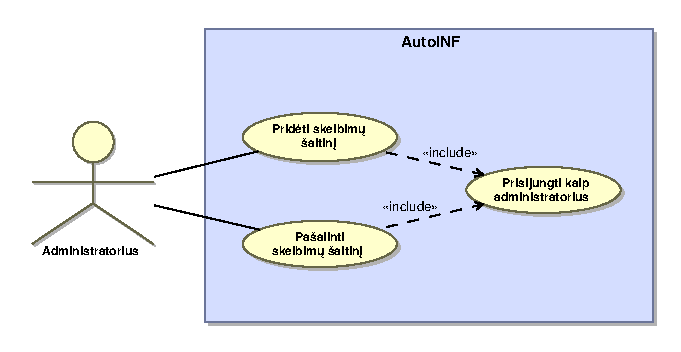
\includegraphics[width=0.7\textwidth]{TikslaiAdministratorius.eps}
			\caption{Sistemos užduočių diagrama iš administratoriaus perspektyvos\label{UseCaseAdmin}}
		\end{center}
	\end{figure}
	\pagebreak
	
	\subsubsection{Administratoriaus prisijungimo reikalavimai}
	\begin{enumerate}[labelindent=10pt,leftmargin=2.2cm]
		\item Sistema užtikrina, kad prisijungimo duomenys suvesti teisingai.
		\item Prisijungus yra perkraunamas pagrindinis langas su prisijungusio administratoriaus interfeisu. 
	\end{enumerate}
		
		\begin{center}
		\captionof{table}{Pagrindinio lango scenarijus, kai administratorius yra prisijungęs\label{UserNotLoggedIn}}		
		\begin{tabular}{ | c | c | c | }
			\hline
			Žingsnis & Aktorius         & Veiklos apibūdinimas \\ \hline
			1        & Aplikacija       & \makecell{Aplikacija paprašo pasirinkti norimą veiksmą: \\ Pridėti skelbimų šaltinį \\ Pašalinti skelbimų šaltinį} \\ \hline
			2        & Administratorius & Administratorius pasirenka veiksmą \\ \hline
			3        & Aplikacija       & Aplikacija įvykdo pasirinktą veiksmą \\ \hline
		\end{tabular}
		\bigskip

		\captionof{table}{Administratoriaus peržiūrėti skelbimų šaltinius scenarijus\label{AdminViewSourcesScen}}
		\begin{tabular}{ | c | c | c | }
			\hline
			Žingsnis & Aktorius         & Veiklos apibūdinimas \\ \hline
			1        & Administratorius & Prisijungia \\ \hline
			2        & Aplikacija       & \makecell{Atidaro pagrindinį langą su administratoriaus interfeisu ir \\ laukia, kol administratorius atliks kokį veiksmą} \\ \hline
			3        & Administratorius & Pasirenka peržiūrėti skelbimų šaltinius \\ \hline
			4        & Aplikacija       & Siunčia užklausą į serverį \\ \hline
			5        & Serveris         & Siunčia užklausą į duomenų bazę \\ \hline
			6        & Duomenų bazė     & Grąžina skelbimų šaltinių sąrašą į serverį \\ \hline
			7        & Serveris         & Grąžina skelbimų šaltinių sąrašą į aplikaciją \\ \hline
			8        & Aplikacija       & Parodo skelbimų šaltinių sąrašą \\ \hline
		\end{tabular}
		\bigskip

		\captionof{table}{Administratoriaus peržiūrėti skelbimų šaltinius scenarijaus plėtiniai\label{AdminViewSourcesScenExtra}}		
		\begin{tabular}{ | c | c | c | }
			\hline
			Žingsnis & Sąlyga         & Veiklos apibūdinimas \\ \hline
			6a       & \makecell{Duomenų bazėje \\ nėra šaltinių} & \makecell{Duomenų bazė grąžina pranešimą, kad \\ skelbimų šaltinių nėra} \\ \hline
		\end{tabular}
		\end{center}
	
	\subsubsection{Administratoriaus skelbimų šaltinio pridėjimo reikalavimai}
	\begin{enumerate}[labelindent=10pt,leftmargin=2.2cm]
		\item Pasirinkęs skelbimų šaltinių pridėjimo funkciją administratorius gali pridėti kokios nors tai svetainės URL ir ši svetainė pridedama į skelbimų šaltinių sąrašą.
		\item Pasirinkęs skelbimų šaltinio šalinimo funkciją administratorius gali pašalinti pasirinktą šaltinį iš sistemos duomenų bazės. 
	\end{enumerate}
		
		\begin{center}
		\captionof{table}{Administratoriaus skelbimų šaltinio pridėjimo scenarijus\label{AdminAddSourceScen}}		
		\begin{tabular}{ | c | c | c | }
			\hline
			Žingsnis & Aktorius         & Veiklos apibūdinimas \\ \hline
			1        & Administratorius & Pasirenka skelbimų šaltinių peržiūros funkciją \\ \hline
			2        & Aplikacija       & Parodo skelbimų šaltinius \\ \hline
			3        & Administratorius & \makecell{Suveda naujo skelbimų šaltinio duomenis ir \\ spaudžia mygtuką „Pridėti šaltinį“ } \\ \hline
			4        & Aplikacija       & Siunčia užklausą į serverį \\ \hline
			5        & Serveris         & Siunčia užklausą į duomenų bazę \\ \hline
			6        & Duomenų bazė     & \makecell{Prideda naują skelbimų šaltinį ir praneša \\ serveriui apie sėkmingą skelbimų šaltinio pridėjimą} \\ \hline
			7        & Serveris         & \makecell{Praneša aplikacijai apie sėkmingą skelbimų \\ šaltinio pridėjimą} \\ \hline
			8        & Aplikacija       & Atnaujina skelbimų šaltinių sąrašą \\ \hline
		\end{tabular}
		\bigskip

		\captionof{table}{Administratoriaus skelbimų šaltinio pridėjimo scenarijaus plėtiniai\label{AdminAddSourceScenExtra}}		
		\begin{tabular}{ | c | c | c | }
			\hline
			Žingsnis & Sąlyga         & Veiklos apibūdinimas \\ \hline
			6a       & \makecell{Nepavyksta \\ pridėti šaltinio} & \makecell{Duomenų bazė grąžina pranešimą apie \\ nesėkmingą skelbimų šaltinio pridėjimą} \\ \hline
		\end{tabular}
		\end{center}
	\pagebreak
	
	\subsubsection{Administratoriaus skelbimų šaltinio pašalinimo reikalavimai}
	\begin{enumerate}[labelindent=10pt,leftmargin=2.2cm]
		\item Pasirinkęs skelbimų šaltinio šalinimo funkciją administratorius gali pašalinti pasirinktą šaltinį iš sistemos duomenų bazės. 
	\end{enumerate}
		
		\begin{center}
		\captionof{table}{Administratoriaus skelbimų šaltinio šalinimo scenarijus\label{AdminRemoveSourceScen}}		
		\begin{tabular}{ | c | c | c | }
			\hline
			Žingsnis & Aktorius         & Veiklos apibūdinimas \\ \hline
			1        & Administratorius & \makecell{Pasirenka skelbimų šaltinių peržiūros \\ funkciją ir pasirenka šaltinio šalinimą} \\ \hline
			2        & Aplikacija       & Siunčia užklausą serveriui \\ \hline
			3        & Serveris         & Siunčia užklausą duomenų bazei \\ \hline
			4        & Duomenų bazė     & \makecell{Pašalina skelbimų šaltinį ir siunčia pranešimą \\ serveriui apie sėkmingai pašalintą skelbimų šaltinį} \\ \hline
			5        & Serveris         & \makecell{Siunčia pranešimą aplikacijai apie \\ sėkmingai pašalintą skelbimų sąrašą} \\ \hline
			6        & Aplikacija       & \makecell{Atnaujina skelbimų sąrašą ir laukia \\ tolimesnių administratoriaus veiksmų} \\ \hline
		\end{tabular}
		\bigskip

		\captionof{table}{Administratoriaus skelbimų šaltinio šalinimo scenarijaus plėtiniai\label{AdminRemoveSourceScenExtra}}		
		\begin{tabular}{ | c | c | c | }
			\hline
			Žingsnis & Sąlyga         & Veiklos apibūdinimas \\ \hline
			4a       & \makecell{Nepavyksta \\ pašalinti šaltinio} & \makecell{Duomenų bazė grąžina pranešimą apie \\ nesėkmingą skelbimų šaltinio pašalinimą} \\ \hline
		\end{tabular}
		\end{center}	
	\pagebreak
	
	\renewcommand{\thesubsection}{NFR\arabic{subsection}}
	\renewcommand*{\theenumi}{\thesubsection.\arabic{enumi}}
	\renewcommand*{\theenumii}{\theenumi.\arabic{enumii}}
	\section*{Nefunkciniai reikalavimai}
	\addcontentsline{toc}{section}{Nefunkciniai reikalavimai}
	\setcounter{subsection}{0}
	
	\subsection{Vidinių interfeisų reikalavimai}
	\begin{enumerate}[labelindent=10pt,leftmargin=2.2cm]
		\item Sistema turi būti suprogramuota Java programavimo kalba.
		\item Sistema bus sukompiliuota laisvai platinamu standartiniu Java kompiliarotiumi.
		\item Sistema veiks Android aplinkoje, versijos pasirinkimas paliekamas programuotojų nuožiūrai.
		\item Programavimo aplinkos pasirinkimas paliekamas programuotojų nuožiūrai.
		\item Duomenims saugoti naudojama PostgreSQL duomenų bazė.
	\end{enumerate}	
	
	%\renewcommand*{\theenumi}{\thesubsubsection.\arabic{enumi}}
	%\renewcommand*{\theenumii}{\thesubsubsection.\theenumi.\arabic{enumii}}
	%\renewcommand*{\theenumiii}{\thesubsubsection.\theenumi.\theenumii.\arabic{enumiii}}
	%\subsection{Veikimo reikalavimai}
	%Šiame skyriuje aprašomi sistemos veikimo reikalavimai.
	
	\subsection{Tikslumo reikalavimai}
	\begin{enumerate}[labelindent=10pt,leftmargin=2.2cm]
		\item Skelbimo kaina atvaizduojama double formatu 2 skačių po kablelio tikslumu ir nėra apvalinama.
		\item Duomenys apie valiutą saugomi double formatu. Skaičių kiekis po kablelio neribojamas.
	\end{enumerate}	
	
	\subsection{Patikimumo reikalavimai}
	\begin{enumerate}[labelindent=10pt,leftmargin=2.2cm]
		\item Įvykus kokiam nors sistemos sutrikimui, sistema turi perkelti vartotoją į prieš tai atliktą žingsnį.
		\item Įvykus sutrikimui sistema neatskleidžia vidinių sutrikimo priežasčių vartotojui (nebent sutrikimas įvyko dėl jo kaltės). Visus sistemos lūžius ir to priežastis sistema saugo duomenų bazėje, prieinamoje tik savininkui ir administratoriui.
		\item Skelbimas vartotojo mėgstamiausiųjų sąraše atsiranda tik tada, kai jis pridedamas į duomenų bazę.
		\item Sistema nebus galima naudotis, kai bus atnaujinama sistemos duomenų bazė.
	\end{enumerate}	
	
	\subsection{Robastiškumo reikalavimai}
	\begin{enumerate}[labelindent=10pt,leftmargin=2.2cm]
		\item Visos klaidos yra saugomos sistemos duomenų bazėje, klaidų registre.
		\item Įvykus nedideliam sutrikimui (pvz., dingsta ryšys su duomenų baze; neatsako skelbimų puslapiai) sistema kartoja paskutinį veiksmą 30 s. Neatsistačius funkcionalumui sistema išsaugo klaidos priežastį duomenų bazėje, atsiprašo vartotojo už nepatogumus ir prašo vartotojo pabandyti naudotis sistema vėliau.
		\item Įvykus rimtam sutrikimui (pvz., atnaujintas skelbimų puslapio HTML kodas; pasikeičia skelbimų nuskaitymo būdas, todėl nebeįmanoma gauti skelbimų informacijos, nors puslapis ir atsako), sistema turi gebėti išimti puslapį iš pasirinkimo galimybių ir užregistruoti veiksmą duomenų bazėje.
		\item Po sistemos sutrikimo tikėtinas atsistatymo laikas yra laikas, reikalingas sistemos perkrovimui.
		\item Sutrikus infrastruktūrai (pvz., duomenų bazei) sistema pradės veikti iš karto, kai infrastruktūra bus sutvarkyta.
	\end{enumerate}	
	
	\subsection{Našumo reikalavimai}
	\begin{enumerate}[labelindent=10pt,leftmargin=2.2cm]
		\item Sistema iš karto turi pranešti vartotojui, kad priėmė paieškos duomenis ir kad paieška yra vykdoma.
		\item Sistema turėtų parodyti pirmąjį užklausos puslapį ne lėčiau kaip per 10 s.
		\item Sistema į vartotojo įvestį turi sureguoti ne lėčiau kaip per 0,5 s.
		\item Užklausų skaičius, kurį maksimaliai be vėlavimo gali atlikti serveris, yra 10 000 per sekundę (nebent sistemos savininko infrastruktūra nėra pakankamai pajėgi).
	\end{enumerate}
	
	\pagebreak
	\renewcommand{\thesubsection}{IR\arabic{subsection}}
	\renewcommand*{\theenumi}{IR\arabic{enumi}}
	\renewcommand*{\theenumii}{\theenumi.\arabic{enumii}}
	\section*{Interfeiso reikalavimai}	
	\addcontentsline{toc}{section}{Interfeiso reikalavimai}
	\setcounter{subsection}{0}
	\begin{enumerate}[labelindent=10pt,leftmargin=2.2cm]
		\item Originali valiuta automatiškai konvertuojama į eurus, bet vartotojas gali pasirinkti, kurią valiutą iš pagrindinių (pagrindinės valiutos pasirenkamos programuotojų atžvilgiu, bet nemažiau kaip 3, iš kurių viena - euras) rodyti.
		\item\label{MainWindowDisplayReq} Pagrindinis langas, kuris atvaizduojamas įjungus programą, yra paieškos langas. 
		\item\label{AdParts} Visi skelbimai sąraše atvaizduojami formatu, kurio pagrindinės dalys yra:
		
		\begin{enumerate}[label=\theenumi.\arabic{enumii}]
			\item Pagrindinė skelbimo nuotrauka,
			\item Automobilio markė,
			\item Automobilio modelis,
			\item Kuro tipas,
			\item Variklio litražas,
			\item Kėbulo tipas,
			\item Kaina.
		\end{enumerate}
		
		\item Paieškos lange turi būti leidžiama pasirinkti skelbimo pagrindinių dalių paieškos filtrus, tačiau galima ir detalesnė paieška.
		\item Detalesnei paieškai turi būti atskiras langas su platesne pasirinkimų specifikacija.
		\item Laukas „Kaina“ ir „Metai“ turi būti leidžiami pasirinkti tipu „Nuo-Iki“, tačiau veikimas privalomas tiek nedetalizavus nė vieno lauko, tiek tik su „Nuo“, tiek tik su „Iki“, tiek su abiejais.
		\item Paieškos tipai (mažiausiai 3, pvz.: automobiliai, motociklai, ratlankiai) turi būti lengvai keičiami skirtukais („Tabs“) pagrindiniame paieškos lange.
		\item Viename paieškos rezultatų lange maksimaliai gali būti 20 skelbimų.
		\item Po 10 skelbimų (jei tiek nėra - sąrašo pabaigoje) turi būti išskirta vieta reklamai. Dydis pasirenkamas programuotojo nuožiūra, tačiau nedidesnis nei skelbimo dydis.
		\item Paieškos rezultatų lango viršuje turi būti rodoma paieškos informacija.
		\item Sistemoje turi būti įdiegta galimybė bet kuriame jos etape grįžti į pagrindinį paieškos langą ir, jei vartotojas yra prisijungęs, į mėgstamiausių skelbimų sąrašo langą (jei vartotojas nėra prisijungęs - į prisijungimo langą). Siūlomas sprendimas - įrankių juosta viršuje visų langų.
		\item Įrankių juostos mygtukai „Mėgstamiausių sąrašas“, „Prisijungimo langas“ ir „Registracijos langas“ turi būtinai būti matomi. Kiti, papildomi mygtukai (pvz.: „Nustatymai“) gali būti pasislėpę po perpildančiu („Overflow“) sąrašu.
		\item Visi skelbimai turi turėti aiškų mygtuką, kuris leis skelbimą pridėti prie mėgstamiausių sąrašo.
		\item Mėgstamiausių sąrašo langas turi turėti mygtuką mėgstamiausių skelbimų pašalinimui.
		\item Šriftų dydis pagrindiniame lange ne mažesnis nei 20 pt, skelbimo formate - ne mažesnis nei 10 pt.
		\item Tarpai tarp eilučių turi būti tokie, kad eilutės nesiliestų viena su kita.
		\item Atsižvelgiant į \ref{MainWindowDisplayReq} punktą vartotojui nedetalizavus paieškos pagrindiniam sistemos veiksmui (paieškai) atlikti užtenka 1 veiksmo - paspausti paieškos mygtuką, kuris turi būti pagrindiniame lange ir turi būti didelis ir gerai matomas.
		\item Sistema neturi būti pritaikyta neįgaliesiems.
	\end{enumerate}
	
\end{document}